
\begin{figure}[t]
    \centering
    \begin{minipage}[b]{\linewidth}
    \centering
    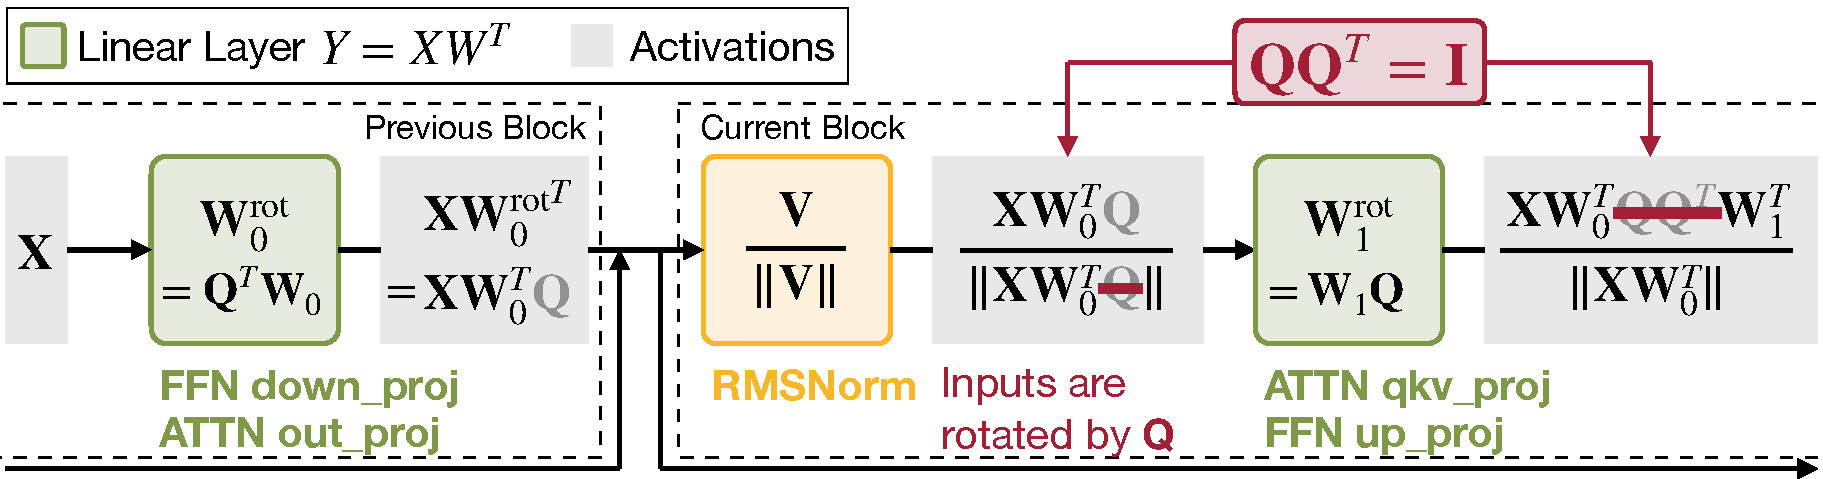
\includegraphics[width=\linewidth]{figure/4-algorithm/rotation.pdf}
    \caption{\textbf{Rotate the block input activations to suppress the outliers}: since rotation is a unitary transformation, the rotation matrix $\mathbf{Q}$ can be absorbed by the weights of the output module in the previous block.}
    \label{fig:alg:other:rotation}
    \end{minipage}
    \begin{minipage}[b]{\linewidth}
    \centering
    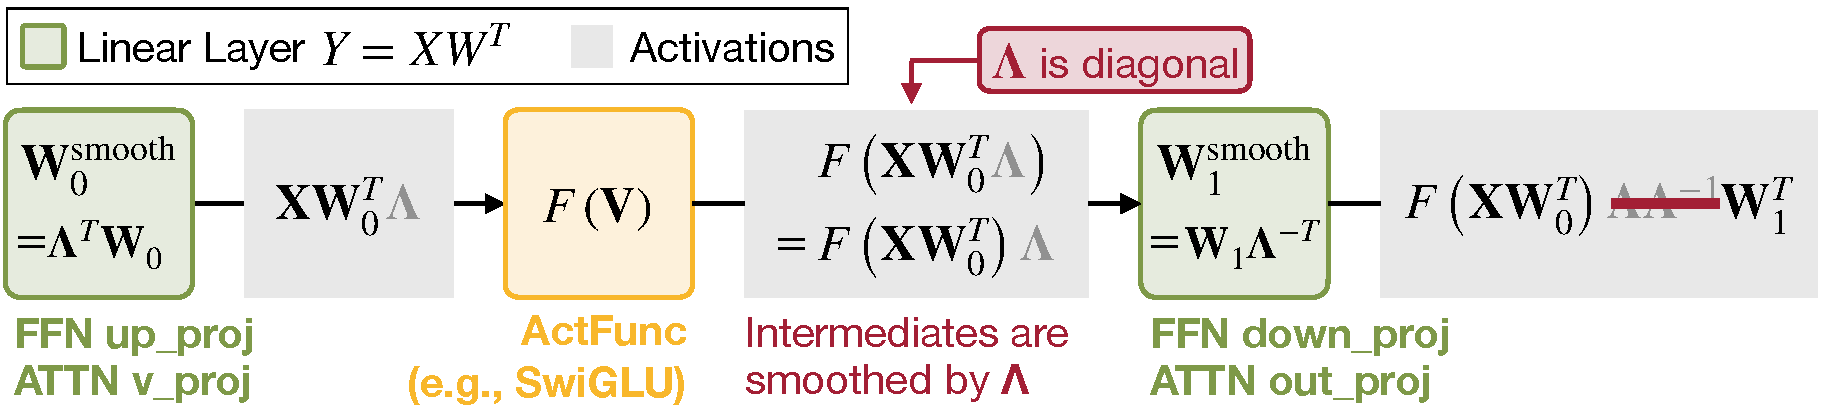
\includegraphics[width=\linewidth]{figure/4-algorithm/smooth.pdf}
    \caption{\textbf{Smooth the block intermediate activations, migrating the quantization difficulty to weights}: since smoothing is channel-independent, the smooth matrix $\mathbf{\Lambda}$ is diagonal and can be absorbed by the weights of the previous modules.}
    \label{fig:alg:other:smooth}
    \end{minipage}
\vspace{-45pt}
\end{figure}
